\documentclass[11pt,a4paper]{article}
\usepackage[british]{babel}

\usepackage{a4wide}
\usepackage{minted}
% \usepackage{xcolor}
% \usepackage{fancyhdr}
\usepackage{graphicx}
% \usepackage{subcaption}
\usepackage{parskip}
\usepackage{amsmath}
\usepackage{amssymb}
\usepackage{wrapfig}
% \usepackage{booktabs}
\usepackage{fancyref}
\usepackage{float}
\usepackage[version=4]{mhchem}
% \usepackage{lipsum}
\usepackage[top=2cm, bottom=2.5cm, left=2.5cm, right=2.5cm]{geometry}
\usepackage{caption} %in order to use "captionsetup"
\usepackage[free-standing-units=true, uncertainty-mode=separate, exponent-product=\cdot]{siunitx} % for consistent handling of SI units
\usepackage[colorlinks=true, pdfstartview=FitV, linkcolor=black, citecolor=black, urlcolor=black]{hyperref} % enable links

% \setlength{\parindent}{0pt}

% \lstset{
%   language=Python,             % Specify the programming language
%   basicstyle=\ttfamily,        % Use a typewriter font for the code
%   keywordstyle=\color{blue},   % Color for keywords
%   commentstyle=\color{green},  % Color for comments
%   stringstyle=\color{red},     % Color for strings
%   numbers=left,               % Line numbers on the left
%   numberstyle=\tiny\color{gray}, % Style of line numbers
%   stepnumber=1,               % Number every line
%   numbersep=5pt,              % Distance of numbers from the code
%   frame=single,               % Put a frame around the code
%   breaklines=true,            % Automatically break long lines
%   showstringspaces=false      % Don’t show spaces in strings
% }

\title{Arago Spot}
\author{Laura Acinapura, Joshua Dreier, Florian Frauenfelder, Johanna Kroker, \\ Davide Plozner and Janik Tavarner}
\date{\today}

\begin{document}

\maketitle

\begin{figure}[h]
    \centering
    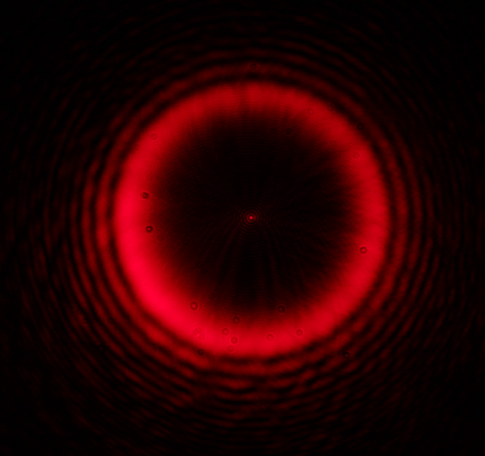
\includegraphics[width=0.5\linewidth]{images/cover-picture.png}
\end{figure}

\begin{abstract}
The goal of this experiment is to reproduce the Arago spot for a spherical object and to observe the diffraction pattern of an ellipse and a square. This is done by measuring the intensity profile of the resulting diffraction pattern. In addition, the dependence of the diffraction pattern on the Fresnel number was explored.
\end{abstract}

% \tableofcontents

% \twocolumn

\vspace{0.75cm}

\section{Introduction}
The Arago spot, also known as the Fresnel spot or Poisson spot, is an interesting phenomenon that was historically used in proving the wave-nature of light. A basic description of the phenomenon is the presence of a bright spot of light in the middle of the shadow of a circular, opaque object. Astonishingly, the bright spot appears at a place where the particle theory of light predicts there to be none, thus disproving the notion that light propagates through space similarly to particles. 
The concept of Huygens-Fresnel principle is foundational in explaining the phenomenon of the Arago spot. It states that any unobstructed part of a wave front can be interpreted as the emission point of a secondary circular wave or wavelet. In this view, the amplitude and direction of the electromagnetic field at any point in space are the superposition of all the wavelets, taking their phase into consideration. 
According to this, the light propagating from the source diffracts at the unobstructed surrounding of the object, where secondary wavelets are emitted. This constitutes the whole of the unobstructed plane around the object, not only the circumference. These wavelets further propagate and are subject to interference. For a circular object, the wavelets are approximately in phase on the optical axis because the optical paths of the light from the source to any point in the unobstructed region near the circumference of the circular shape and to the point on the optical axis are nearly identical. For this reason, it is important to have an approximate point source of coherent light in order to observe the Arago spot.

Consider a point in the unobstructed object plane, with a distance \(r := \sqrt{x^{2} + y^{2}}\) from the optical axis and a distance \(\sqrt{r^{2} + s^{2}}\) from the detector. In cylindrical coordinates, the time-independent part of the electric field \(U(r)\) at the detector \(P\) can be expressed as an integral over all possible point sources.

\[U(P) \propto A_{0} \int_{R}^{\infty} r \int_{0}^{2\pi} \frac{e^{ik\sqrt{s^{2} + r^{2}}}}{\sqrt{s^{2} + r^{2}}} \frac{e^{ik\sqrt{s^{2} + r^{2}}}}{\sqrt{s^{2} + r^{2}}} \, \mathrm{d}\theta \, \mathrm{d}r = 2\pi A_{0} \int_{R}^{\infty} \frac{re^{2ik\sqrt{s^{2} + r^{2}}}}{s^{2} + r^{2}} \, \mathrm{d}r\]

Using the substitution

\[u = 2k\sqrt{s^{2} + r^{2}} \implies \mathrm{d}u = \frac{2kr}{\sqrt{s^{2} + r^{2}}} \, \mathrm{d}r,\]

we get

\[U(P) \propto 2\pi A_{0} \int_{2k\sqrt{s^{2} + R^{2}}}^{\infty} \frac{1}{u} e^{iu} \, \mathrm{d}u \approx \frac{\pi iA_{0}}{k\sqrt{s^{2} + R^{2}}} e^{2ik\sqrt{s^{2} + R^{2}}} \neq 0,\]

where in the last step, we use the approximation:

\[\int_{a}^{\infty} \frac{1}{x} e^{ix} \, \mathrm{d}x \approx \frac{i}{a} e^{ia}\]

for \(a\) large enough, which holds for \(R \gg \lambda\).

\begin{wrapfigure}{r}{0.4\textwidth}
    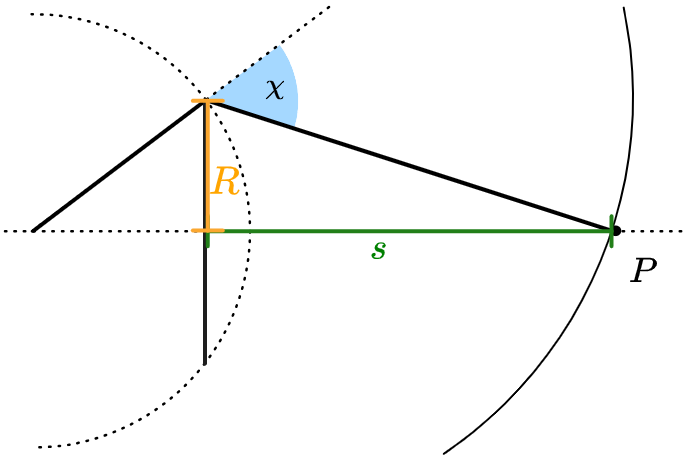
\includegraphics[width=1\linewidth]{images/diffraction-angle.png}
    \caption{Simplified representation and angle of diffraction $\chi$}
\end{wrapfigure}

To calculate the intensity correctly, we need to assume in total \(s \gg R \gg \lambda\).
Including the angle of diffraction \(\chi\) we get a more accurate expression for the spatial part of the wave \cite{KTHReport}:

\[U(P) = \frac{A_{0}i}{2\lambda} \int_{R}^{\infty} r \int_{0}^{2\pi} \frac{e^{ik\sqrt{s^{2} + r^{2}}}}{\sqrt{s^{2} + r^{2}}} \frac{e^{ik\sqrt{s^{2} + r^{2}}}}{\sqrt{s^{2} + r^{2}}} (1 + \cos \chi) \, \mathrm{d}\theta \, \mathrm{d}r,\]

from which we get the intensity:

\[I(P) = \frac{s^{2}}{s^{2} + R^{2}} I_{0} \xrightarrow{s \gg R} I_{0}\]
\\\vspace{0.5cm}

To achieve an optimal result, the Fresnel number \(F\) should satisfy the following inequality:

\[F := \frac{4R^{2}}{s\lambda} \gtrsim 1\]

When \(F \ll 1\), near-field diffraction is a dissatisfactory approximation and Fraunhofer diffraction should be considered.

More complex diffraction patterns appear for different shapes, e.g. an evolute for an ellipse. In general, the phenomenon of the Arago spot is rather sensitive to irregularities in the circumference of the shape like the surface roughness. The deviation should not exceed \(\SI{10}{\percent}\) of the Fresnel zone to see an ideal spot. The Fresnel zone for a \(\SI{4}{mm}\) disk is about \(\SI{77}{\micro m}\). \cite{WikipediaAragoSpot}

To better understand the principles that were presented, a simulation that models the diffraction of light on different shapes was created. The simulation was built with Python and the whole of the code can be found in the appendix. The simulation was also used to make theoretical predictions about the diffraction patterns of different shapes and Fresnel numbers that were encountered in the experimentation. 

\section{Experiment Setup}
The base of the experimental setup consists of two optical mounting rails. The smaller one holds the laser as the source of light, and the first of two mirrors, which are used to precisely direct the beam of light onto the object. A beam of light is emitted by a laser instrument with a wavelength of \(\lambda = \SI{635}{nm}\). The larger mounting rail is placed adjacent to the smaller one and holds the second mirror, which directs the beam of light through an iris diaphragm onto the object in the object holder. The diffracted light from the object is then captured by a Canon EOS 1300D, mounted at the end of the larger rail.  In order to decrease the high intensity of the beam of light a beam splitter was placed between the laser and the first mirror.  
The diameter of the beam of light was larger than the diameter of the metal bead (\(\SI{2.5}{mm}\)) with which the dependence of the Arago spot on the Fresnel number was examined. 
In order to change the Fresnel number, the optical distance between the laser and the object was kept constant while the distance between the object holder and the camera mount was decreased from \(\SI{94+-0.1}{cm}\) down to \(\SI{6+-0.1}{cm}\). 

\begin{figure}[h]
    \centering
    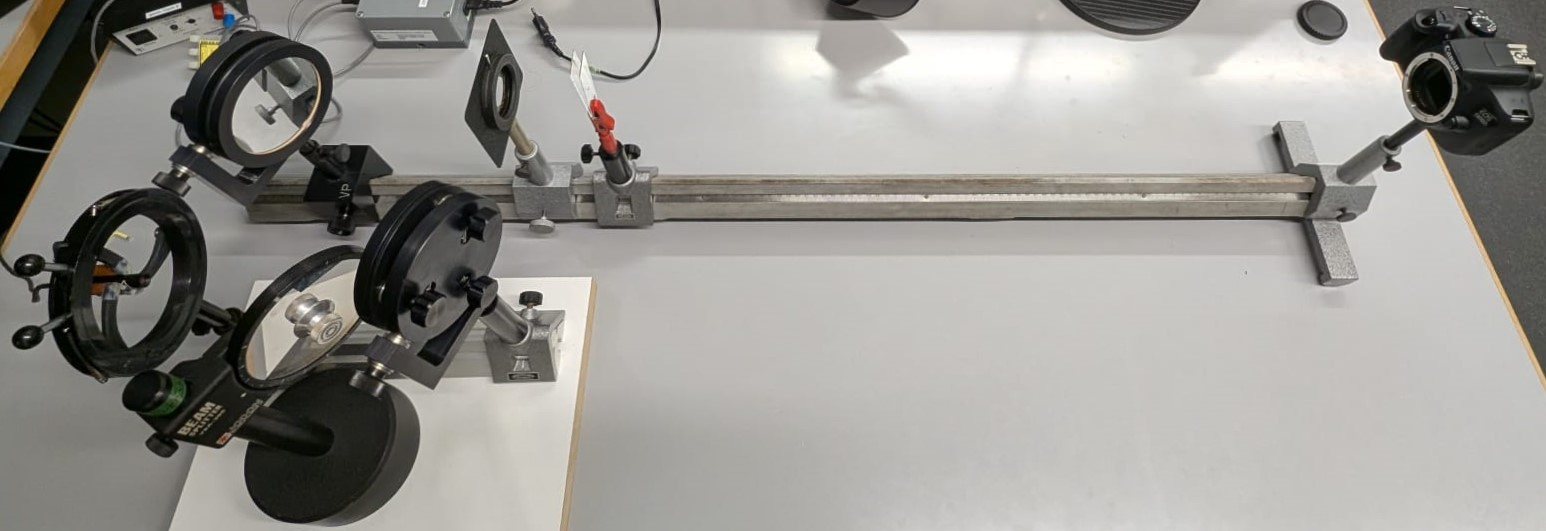
\includegraphics[width=0.7\linewidth]{images/Setup Arago Spot.jpeg}
    \caption{Experimental setup to observe the Arago spot, created by a metal bead}
\end{figure}

For resolving the diffraction pattern of the ellipse, the beam of light had to be slightly widened with a diverging lens before the object holder and then refocused again with a converging lens before the camera. 

\section{Results and data analysis}
\label{sec:results}

\subsection{Visualizing the Arago Spot}
Our first goal was to visualize the Arago spot and compare its intensity profile with our theoretical simulations. We were able to easily see and take pictures of the diffraction pattern on our main set-up, where the red laser (\(\lambda = \SI{635}{nm}\)) was shined on a \(\SI{2.5}{mm}\) sphere, initially positioned at a distance of \(\SI{94.7}{cm}\) from the camera sensor. This set-up corresponds to a Fresnel number of \(F = 10.88\). A post-processed picture of the resulting interference pattern, next to its corresponding computer simulation, is shown in Fig.~\ref{fig:Arago spot}. Pictures where captioned in RAW mode, which allowed us to directly retrieve the intensity value of each pixel. Additionally, a Gaussian filter with \(\sigma = 1\) was applied in post-processing, to get rid of mosaicing effects due to camera artifacts.

\begin{figure}[H]
    \centering
    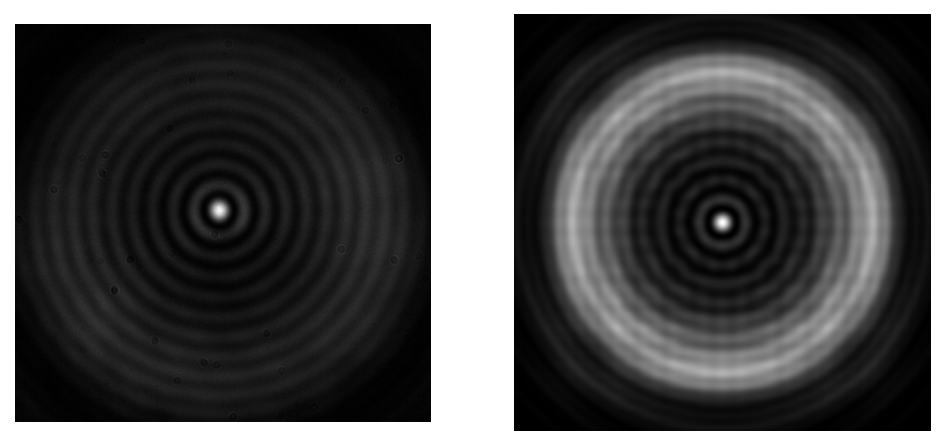
\includegraphics[width=0.5\linewidth]{images/Arago-Spot.pdf}
    \caption{Diffraction pattern at \(F = 10.88\). On the left the picture, on the right the computer simulation. A bright spot is present at the center of the shadow: the Arago spot}
    \label{fig:Arago spot}
\end{figure}

\begin{figure}[h]
    \centering
    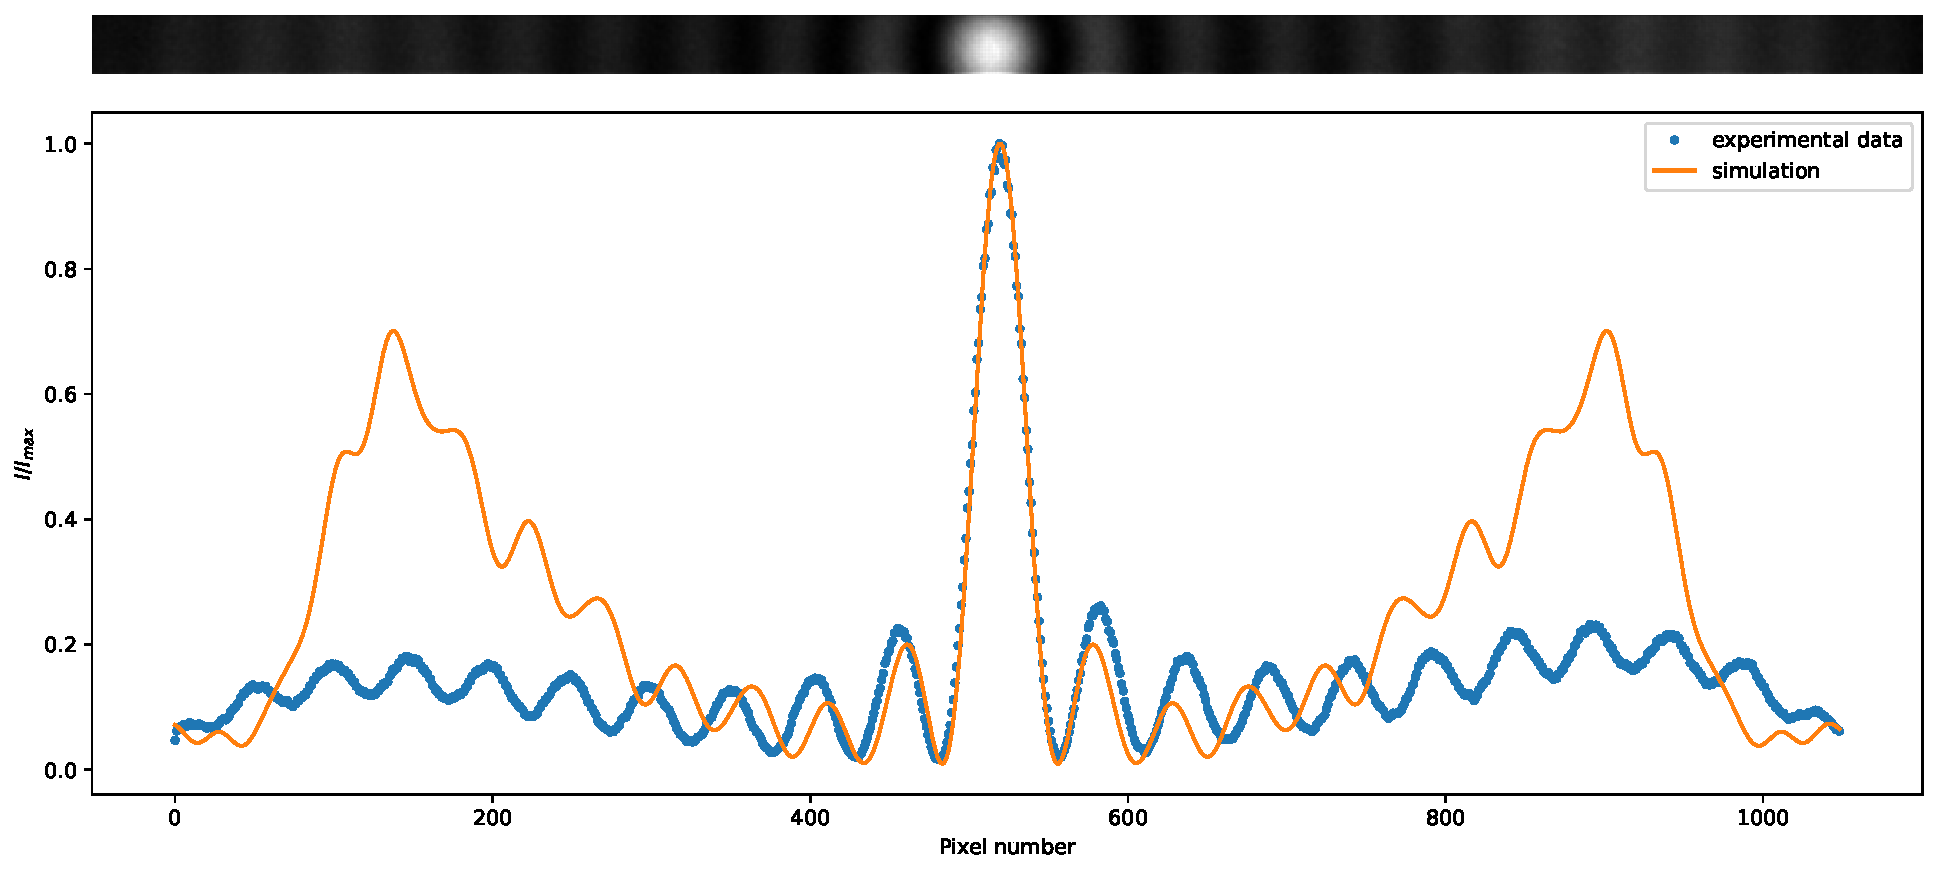
\includegraphics[width=\linewidth]{images/Intensity-profile.pdf}
    \label{fig:Intensity profile}
    \caption{Normalized intensity distribution of the diffraction pattern, averaged over the central cutout of 34 pixels displayed at the top and plotted against the intensity from the simulation.}
    \label{fig:Arago-Spot and Intensity profile}
\end{figure}

The intensity profile of a central strip is represented in Fig.~\ref{fig:Arago-Spot and Intensity profile} together with the simulation values. The plot highlights the fact that the Arago spot is indeed the brightest spot of the diffraction pattern. While the experimental data well overlaps with the simulation near the center of spot, the two distributions differ at the edge of the outer diffraction ring, where from the model we would expect the intensity to increase again. Furthermore, an equivalent number of fringes is observable in the two plots, despite their position being different.

\subsection{Fresnel number dependency}
After having successfully been able to image the Arago spot, we proceeded to investigate the relationship between the diffraction pattern and the Fresnel number. 

The calculations that predict the formation of a central, bright spot rely on approximations applicable when \(F \gtrsim 1\); for \(F \ll 1\) we fall back in the Fraunhofer limit while for \(F \gg 1\) in the geometric optics limit.
More specifically, we were interested in finding out how big \(F\) can actually become before we stop seeing the Arago spot at all. We varied \(F\) in a way that would minimize the changes we had to implement in our setup, that is by keeping the sphere size and the wavelength of the laser constant, and by changing instead the distance between the obstacle and the imaging device. 

We took 49 consecutive images of the interference pattern, decreasing the distance between the sphere and the camera sensor by \(\SI{2}{cm}\) each time, with the exception of the last five photos, which where taken at \(\SI{1}{cm}\) decrements from each other.

\begin{figure}[H]
    \centering
    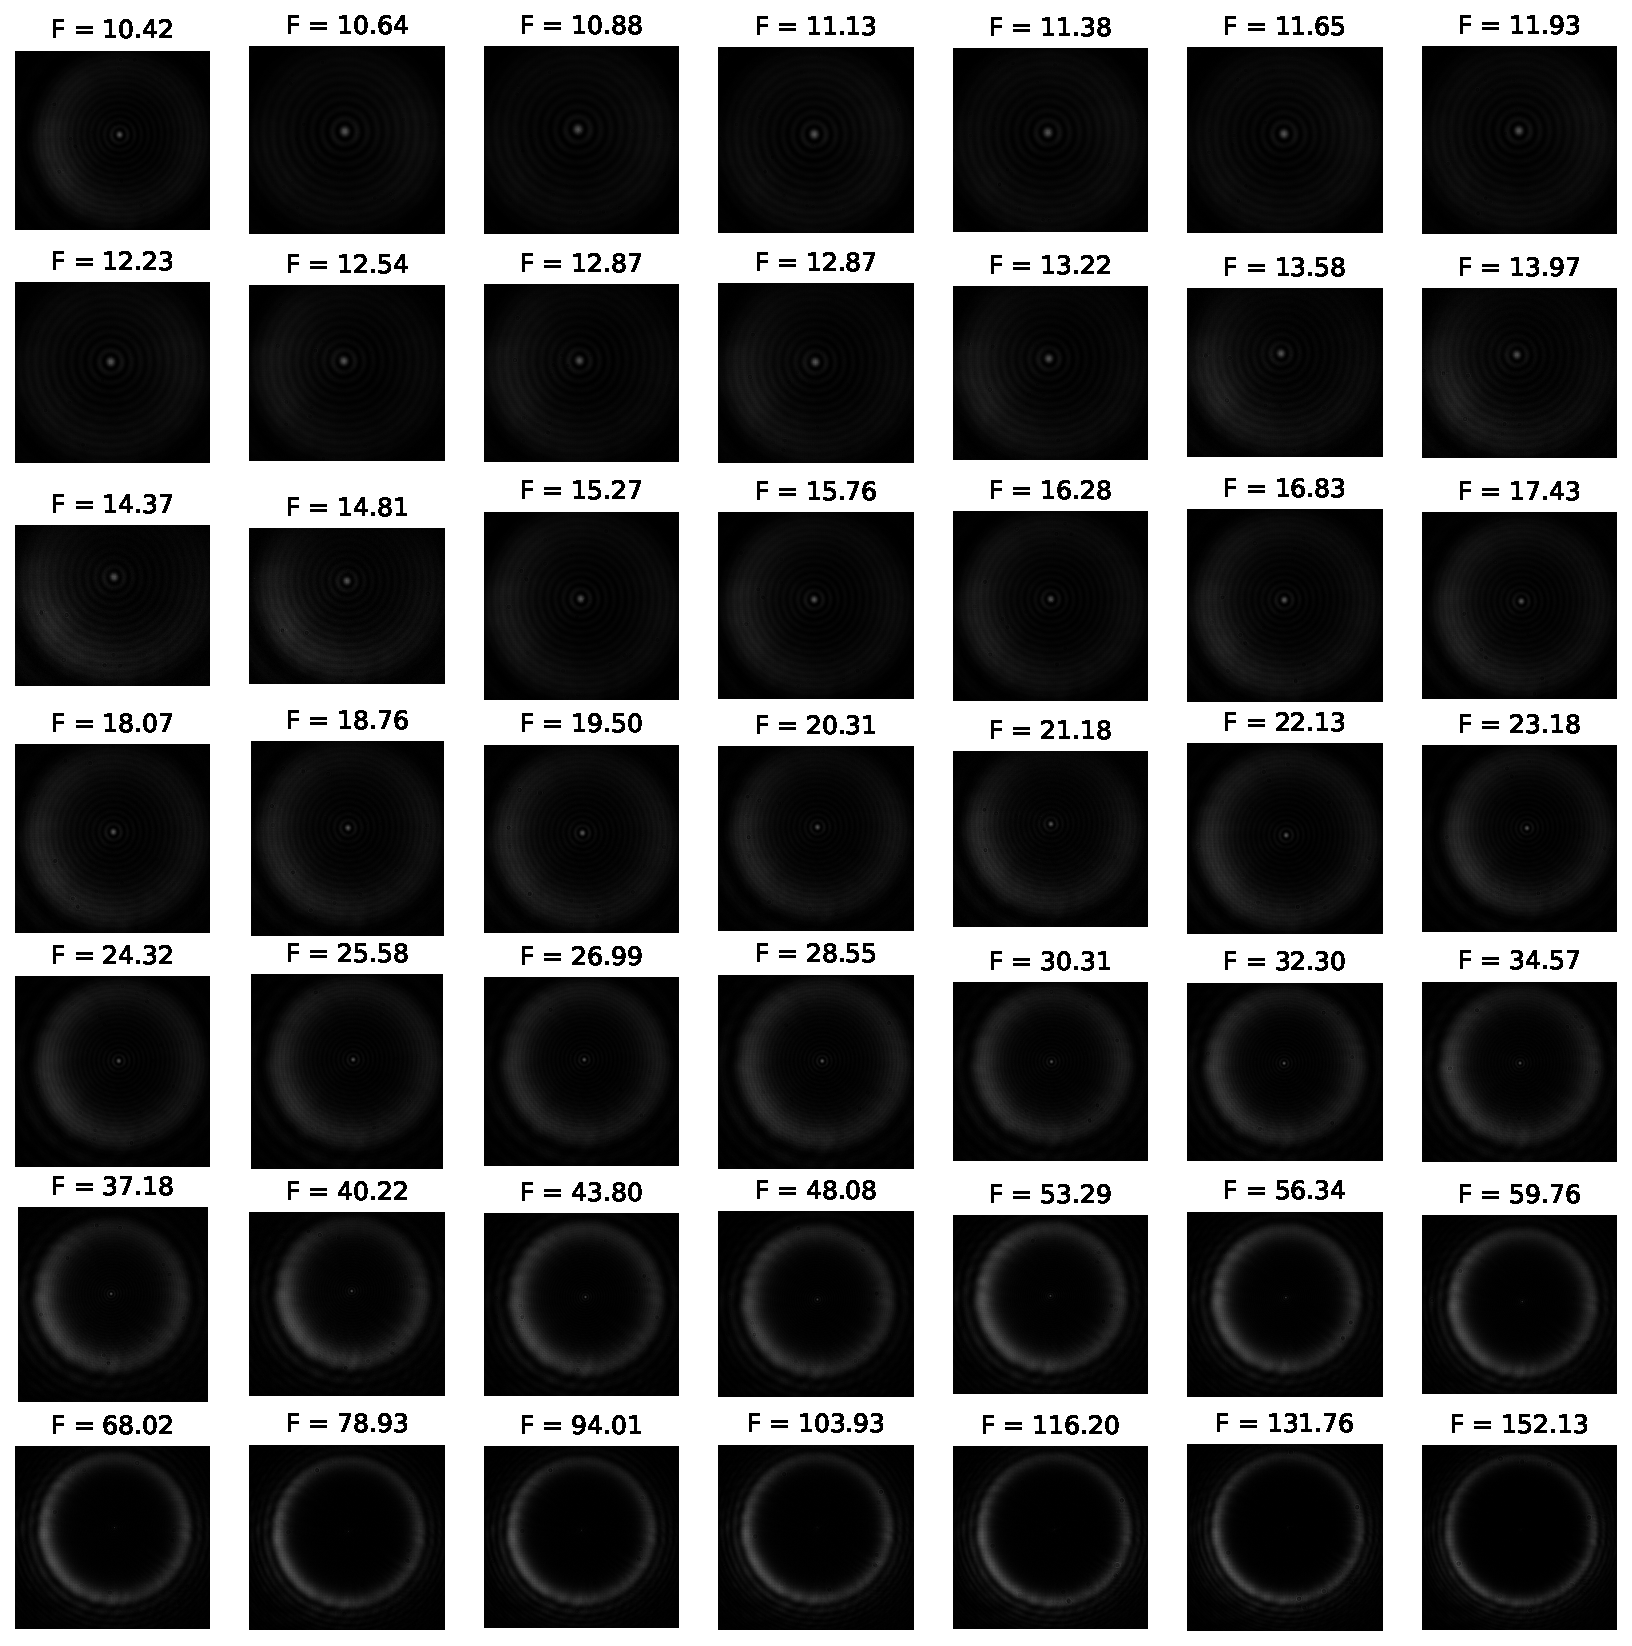
\includegraphics[width=0.8\linewidth]{images/Fresnel-grid.pdf}
    \caption{Diffraction pattern observed at different values of the Fresnel number \(F\)}
    \label{fig:fresnel-number-grid}
\end{figure}

\begin{figure}[H]
    \centering
    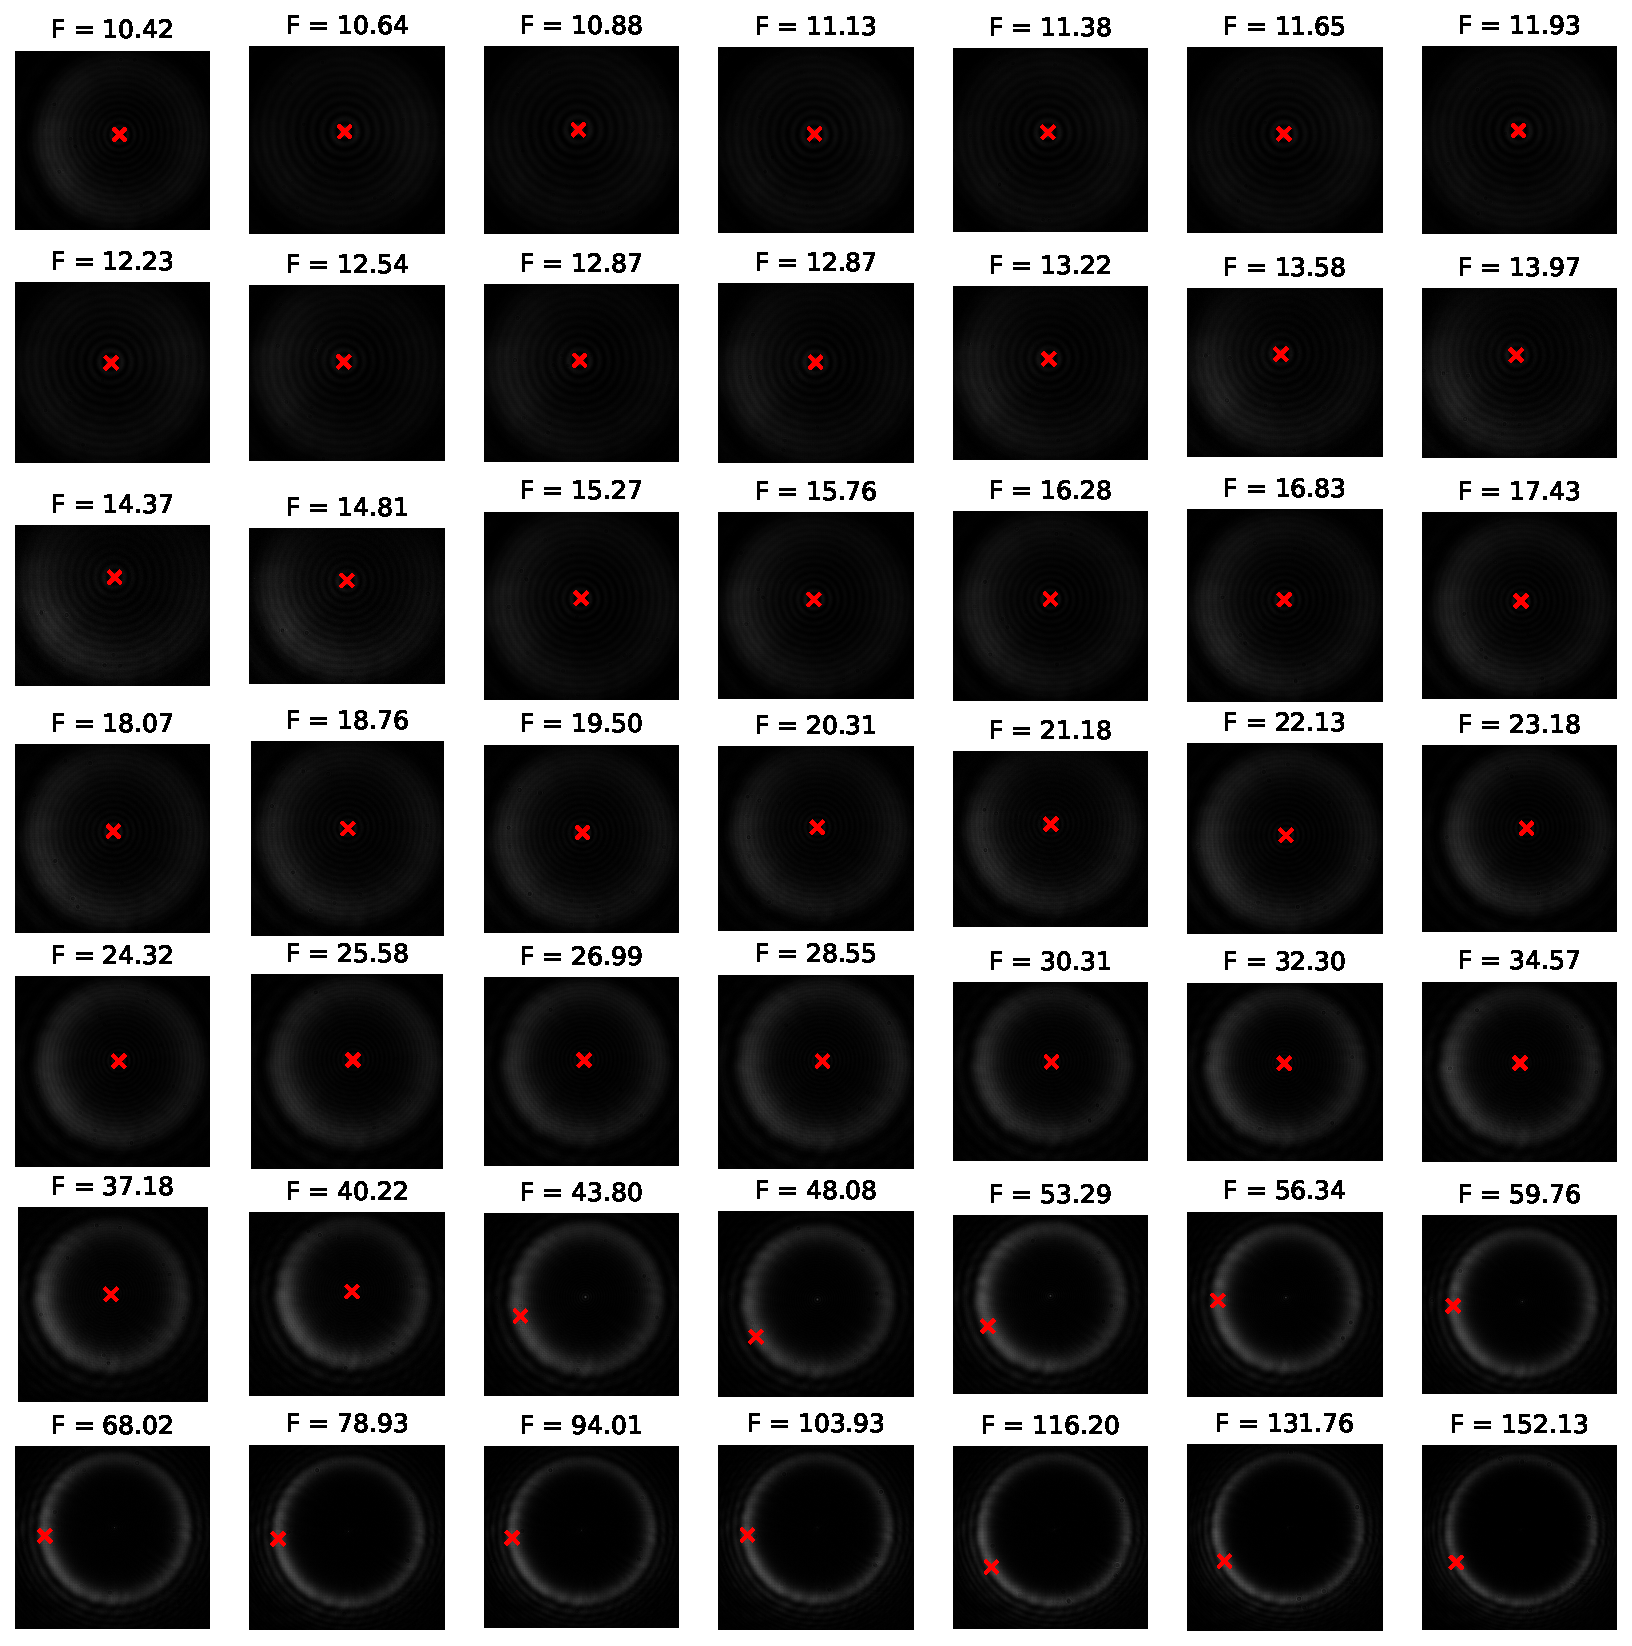
\includegraphics[width=0.35\linewidth]{images/Fresnel-grid-brightest-spot.pdf}
    \caption{Diffraction pattern observed at different values of the Fresnel number \(F\). A red cross is placed over the brightest pixel: the Arago spot is the brightest spot of the shadow until \(F = 43.80\)}
    \label{fig:fresnel-grid-highlighted-spot}
\end{figure}

From Fig.~\ref{fig:fresnel-number-grid} we can see that the Arago spot becomes progressively less visible as \(F\) increases, being virtually undetectable in the last four pictures, for \(F > 94.01\).

Not only Poisson's calculations predicted a bright spot to appear at the center of the shadow of a circular object, but the Arago spot is also supposed to be the brightest spot of the interference pattern. As Fig.~\ref{fig:fresnel-grid-highlighted-spot} clearly highlights, this is the case for \(F < 43.80\), beyond that the error deriving from the approximation becomes too big and the spot fades away.

\subsection{Deviation from circularity}

\begin{figure}[H]
    \centering
    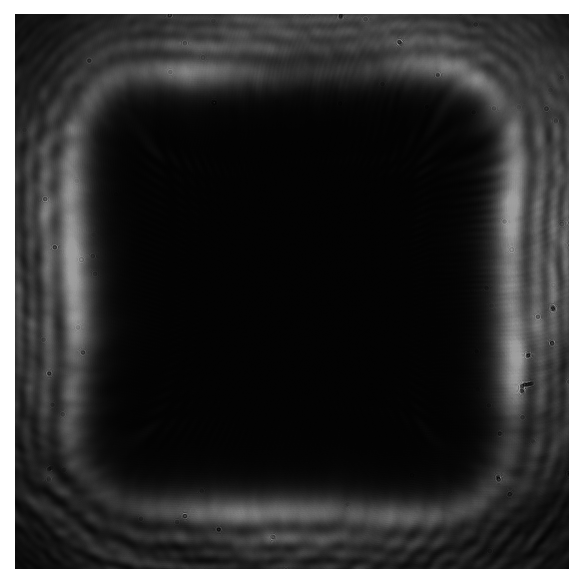
\includegraphics[width=0.3\linewidth]{images/square.pdf}
    \caption{Shadow cast by a square obstacle: no bright central spot is visible}
    \label{fig:square}    
\end{figure}

Much of the literature and calculations around the Arago spot focuses on its existence and properties for a perfectly smooth, circular object. We naturally asked ourselves if and how the spot would appear in the shadows of different obstacles. Apart from the sphere, we 3D printed two additional shapes -- a square and an ellipse -- that we could test on our experimental set-up and compare with the computer simulations.

Agreeing with our simulation, Fig.~\ref{fig:square} displays no Arago spot for the shadow of a square obstacle while Fig.~\ref{fig:ellipse} portrays the faint but nevertheless visible evolute-shaped Arago spot for an ellipse.

\begin{figure}[H]
    \centering
    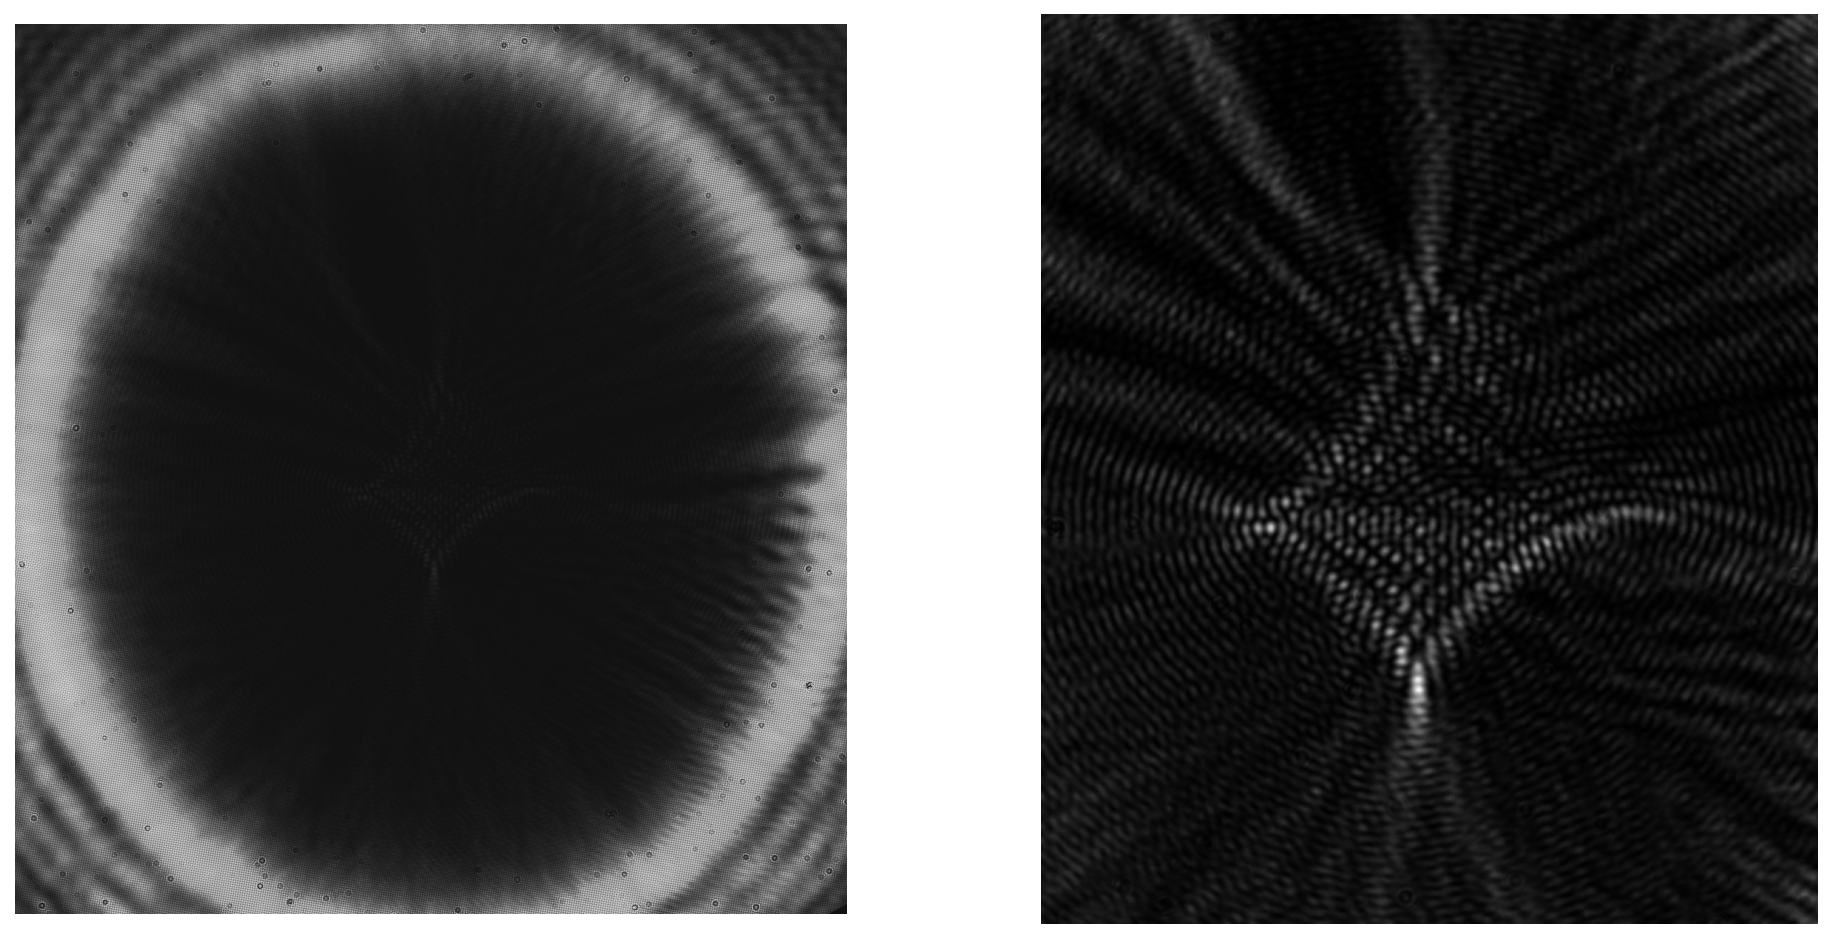
\includegraphics[width=0.6\linewidth]{images/ellipse.pdf}
    \caption{Diffraction pattern created by an ellipse-shaped obstacle. On the right a close up of center of the shadow is shown: the Arago spot created by an ellipse has a diamond-like shape called astroid, that is the evolute of an ellipse.}
    \label{fig:ellipse}
\end{figure}

\vspace{1px}
\section{Discussion}
Our experimental setup was overall functional, allowing us to clearly visualize the Arago spot and  qualitatively confirm all our theoretical predictions, providing results that generally agree with the computer simulations and calculations. Nevertheless, it was also prone to manual mistake when it comes to the alignment of all the components along the optical path, which led it to be quite imprecise on a quantitative level. The laser was not perfectly aligned with the sphere; this mainly impacted the intensity profile of the interference pattern on the outer ring, which was largely skewed on the left for most pictures. Moreover, the discrepancy between the experimental data and the simulation visible in Fig.~\ref{fig:Arago-Spot and Intensity profile} can also be attributed to the fact that our laser was only slightly diverging without any additional use of diverging lenses, being able to barely cover the entire surface of the \(\SI{2.5}{mm}\) diameter sphere, while on the other hand for the simulations a perfectly diverging point source is assumed. 

Furthermore, we only later realized during post-processing that the camera sensor was dirty and some of the dust particles are in fact visible on the pictures. While it would have definitely been better to clean the camera before starting the measurements, this did not end up impacting the effects we were investigating. 

\section{Conclusion}
In this experiment, we successfully observed the Arago spot and studied its diffraction pattern at varying Fresnel number and for different shapes. By illuminating a spherical object with a coherent light source and capturing the resulting diffraction pattern, we confirmed the theoretical prediction that a bright central spot appears in the object's shadow due to constructive interference. The measured intensity profile of the Arago spot was compared with numerical simulations, showing good agreement in the central region but minor deviations near the outer diffraction rings.
Furthermore, by systematically varying the Fresnel number, we explored the transition between the near-field and geometric optics diffraction regimes. Our results indicated that the Arago spot remains the brightest point in the diffraction pattern up to a certain threshold of the Fresnel number, beyond which geometric optics effects dominate, and the spot disappears. Additionally, we examined diffraction patterns for objects of different shapes, such as square, for which no spot was detected, and an ellipse, which exhibited an interesting diamond-shaped interference pattern called evolute. 

% \onecolumn

\newpage

\begin{thebibliography}{99}
\bibitem{KTHReport}
Bergström, P., Eriksson, J. B. (2015): \textit{Capturing the Arago spot using white light} (with help from M. Swillo G. Björk). KTH, Modern Physics SH1012.
\bibitem{WikipediaAragoSpot}
Wikipedia contributors. (2025, March 16). \textit{Arago spot}. Wikipedia, The Free Encyclopedia. Retrieved March 17, 2025, from \url{https://en.wikipedia.org/wiki/Arago_spot}
\end{thebibliography}

\appendix
\section{Python Simulation Code}
\inputminted[linenos,breaklines,frame=single]{python}{images/code.py}

\end{document}
